\documentclass[report,gutter=10mm,fore-edge=10mm,uplatex,dvipdfmx]{jlreq}
\usepackage{lmodern}
\usepackage{amssymb,amsmath}
\usepackage{ifxetex,ifluatex}
\usepackage{actuarialsymbol}
\usepackage[]{natbib}
\RequirePackage{plautopatch}

% maru suji ① etc.
\usepackage{tikz}
\newcommand{\cir}[1]{\tikz[baseline]{%
\node[anchor=base, draw, circle, inner sep=0, minimum width=1.2em]{#1};}}

\usepackage{comment}

\begin{comment}

\ifnum0\ifxetex1\fi\ifluatex1\fi=0 % if pdftex
  \usepackage[T1]{fontenc}
  \usepackage[utf8]{inputenc}
  \usepackage{textcomp} % provide euro and other symbols
\else % if luatex or xetex
  \usepackage{unicode-math}
  \defaultfontfeatures{Scale=MatchLowercase}
  \defaultfontfeatures[\rmfamily]{Ligatures=TeX,Scale=1}
\fi
% Use upquote if available, for straight quotes in verbatim environments
\IfFileExists{upquote.sty}{\usepackage{upquote}}{}
\IfFileExists{microtype.sty}{% use microtype if available
  \usepackage[]{microtype}
  \UseMicrotypeSet[protrusion]{basicmath} % disable protrusion for tt fonts
}{}
\makeatletter
\@ifundefined{KOMAClassName}{% if non-KOMA class
  \IfFileExists{parskip.sty}{%
    \usepackage{parskip}
  }{% else
    \setlength{\parindent}{0pt}
    \setlength{\parskip}{6pt plus 2pt minus 1pt}}
}{% if KOMA class
  \KOMAoptions{parskip=half}}
\makeatother
\usepackage{xcolor}
\IfFileExists{xurl.sty}{\usepackage{xurl}}{} % add URL line breaks if available
\IfFileExists{bookmark.sty}{\usepackage{bookmark}}{\usepackage{hyperref}}
\hypersetup{
  hidelinks,
  pdfcreator={LaTeX via pandoc}}
\urlstyle{same} % disable monospaced font for URLs
\usepackage{longtable,booktabs}
% Correct order of tables after \paragraph or \subparagraph
\usepackage{etoolbox}
\makeatletter
\patchcmd\longtable{\par}{\if@noskipsec\mbox{}\fi\par}{}{}
\makeatother
% Allow footnotes in longtable head/foot
\IfFileExists{footnotehyper.sty}{\usepackage{footnotehyper}}{\usepackage{footnote}}

\end{comment}
%\makesavenoteenv{longtable}
\setlength{\emergencystretch}{3em} % prevent overfull lines
\providecommand{\tightlist}{%
  \setlength{\itemsep}{0pt}\setlength{\parskip}{0pt}}
\setcounter{secnumdepth}{-\maxdimen} % remove section numbering

\author{kazuyoshi}
\date{}

\newcommand{\problem}[1]{\subsubsection{#1}\setcounter{equation}{0}}
%\newcommand{\answer}[1]{\subsubsection{#1}}
\newcommand{\answer}[1]{\subsubsection{解答}}

%Pdf%\newcommand{\wakumaru}[1]{\framebox[3zw]{#1}}
\newcommand{\wakumaru}[1]{#1}





\begin{document}
\chapter{保険2第5章 事業費の管理・分析}
\section{5.1 アクチュアリーと事業費管理}
\section{5.2 事業費}
\problem{H6 生保2問題 2(1)}
損益計算書を作成する際、事業費を計上するに当たって準拠すべき会計原則を列挙し、簡潔に説明
せよ。
\answer{}
\noindent①発生主義

企業会計原則において「すべての費用及び収益は、その支出及び収入に基づい
て計上し、その発生した期間に正しく割当てられるように処理しなければならな
い。ただし、未実現収益は、原則として、当期の損益計算に計上してはならない。」
と規定している。これを発生主義の原則と言い、重要な会計上の認識基準である。

\noindent②実現主義

企業会計原則において「売上高は、実現主義の原則に従い、商品等の販売又は
役務の給付によって実現したものに限る。」と規定している。これを実現主義の
原則と言い、重要な会計上の認識基準である。

\noindent③費用収益対応の原則

企業会計原則において「費用及び収益は、その発生源泉に従って明瞭に分類し、
各収益項目とそれに関連する費用項目とを損益計算書に対応表示しなければなら
ない。」と規定している。

この様な計上原則に則って具体的に事業費を計上・確定する際に留意すべき事
項として、「未払事業費」や「繰延資産」などがある。

「未払事業費」とは、事業費として支出すべき金額で、既に支払期限の到来し
ているもののほか、支払期限は未到来であっても費用収益対応の原則に照し、当
期に計上した収益に対応して支出すべき事業費のうち、未払となっているもので
ある。

「繰延資産」とは、適正な期間損益計算を行うために、
「既に支払われた費用
で将来の期間に影響する特定の費用」を当期の事業費計上の対象外として除外す
るとともに、いわゆる「資産」として繰延経理するものである。

\problem{H7 生保2問題 1(1)}
「広義の事業費」として「事業費」にプラスして考えるべき費用を 2 つ挙げ、その理由を説明せよ。
\answer{}
\noindent 減価償却費(営業関係)

一般に固定資産は、時の経過等によりその価値が減少していくものであること
から、取得年度のみの費用とはせず、費用配分の原則に従って固定資産の取得原
価を各期間に割当て、当期中に目減りした分だけを合理的に算出して当期の費用
とするものだからである。

\noindent 退職給与・退職年金引当金繰入額

退職給与等は現実に支給したときにはじめて発生するものではなく、退職給与
等支給規定の定めるところに従って、従業員の勤務年数の経過につれて毎年累加
的に発生するものであることから、支給年度のみの費用とはせず、毎年の発生額
を毎年の費用とするとともに、その金額を負債性引当金として計上するものだか
らである。

他に填補損、営業関係の税金などがある。

\problem{H16 生保2問題 4(2)①、H12 生保2問題 2(3)①、H4 生保2問題 2(1)}
事業費分析における予定事業費枠の意義と役割について説明せよ。
\answer{}
\noindent{} 1)意義\\
保険料の中にその一部として予め組み込まれた予定事業費を財源として事業運営を行っ
ているという考え方に立って、事業費支出を予定事業費の範囲内、すなわち数理的に計
算される一定の事業費許容枠、に止める様コントロールする。\\
予定事業費枠に対する比率(事業費率)をより逓減させて行くよう経営努力を図ること
によって、契約者負担の軽減を図っていく。

\noindent 2)役割\\
事業費支出を統制するための事業費支出許容限度を示すことから、特に予定事業費統制
に役立てることができる。\\
事業費率の分母として用い、同一会社での事業費効率を年度別に比較したり、他社との
事業費効率の比較を行うことを可能にならしめる。事業費効率を低める(改善する)こ
とにより、経営の合理化を目指す。\\
一定期間内の剰余を利源別に分析する際に中間項目として用いる。これにより、費差損
益・死差損益等を算出し、利源別配当の各財源計算を可能にならしめる。

\problem{(参考)H6 生保2問題 1(3)}
減価償却資産とは何かを説明し、生命保険会社における当該資産を 3 点列挙せよ。
\answer{}
減価償却資産とは、固定資産のうち取得価格が20万円(☆)以上で耐用年数が
1年以一上のものをいう。ここで、固定資産とは使用や時の経過などに伴って価値が
減少していく資産で、\\
①有形減価償却資産(建築物、船舶等)、\\
②無形減価償却資産(特許権等)などがある。

ただし、有形減価償却資産のうち価値の減少しない土地等は減価償却の対象にはならない。
減価償却の方法としては、定額法・定率法なとがあり、
資産の種類、構造、用途等に応じて耐用年数および償却率が定められている。
生命保険会社における当該資産を列挙すると、社屋、社有車、コンピュータ
ー、複写機などがある。

(☆)教科書では取得価格10万円以上となっている為どちらも正解扱いとした。

\section{5.3 予算制度と事業費}
\section{5.4 予定事業費枠と事業費分析}
\problem{2019 生保2問題 3(2)①、H23 生保2問題 2(2)、H19 生保2問題 3(2)②、H17 生保2問題 2(3)、H12 生保2問題 2(3)②、H9 生保2問題 2(3)、H6 生保2問題 1(4)、H1 生保2問題 1(4)}
\vspace{1zh}
予定事業費枠における「蔵銀枠」、「利源枠」、「純保枠」の考え方、
事業費統制の基準として採用する際のメリット・デメリットについて、簡潔に説明しなさい。

\answer{}
\noindent <蔵銀枠>\\
契約初年皮に予定新契約費をすべて費消し、これを全保険期間にわたって償却すると考えて計
算した予定事業費枠。初年度に保険金額比例の予定新契約費が全額収入され、以後は収入され
ないと考える。\\
メリット \\
初年度に販売経費の多くが支出される保険金杜の事業費支出の形態とリンクしているため、単
年度業績により事業費率が左右されにくい。\\
デメリット\\
α全額を初年度に費消するという前提が事業費コントロールの指標として甘いという意見があ
る。特に、保険料収入を超えて予定新契約費が計上されることがある点で注意が必要。\\
予定事業費枠の水準が単年度業績によって大きく変動する。\\

\noindent<利源枠>\\
予定新契約費のうち一定割合を契約初年度に費消し、それを一定期間で償却すると考えて計算
した予定事業費枠。契約初年度に費消する予定新契約費の一定割合をチルメル歩合、償却期間
をチルメル期間という。\\
メリット \\
解約控除を考慮すれば、財源対応が実態に近い。\\
保険料収入を限度とした枠計上。\\
業界共通の尺度として採用されている。\\
デメリット\\
チルメル期間経過後、付加保険料が大きくなる点が不自然。\\
2年目以降チルメル期間内の予定新契約費αが通常マイナスとなる。\\

\noindent<純保枠>\\
付加保険料が毎年一定であるとして計算した予定事業費枠。\\
メリット \\
平準純保険料式の責任準備金を積立てる場合、財務会計上の財源対応がとれている。\\
予定事業費枠の水準が単年度の業績に左右されず安定的。\\
デメリット\\
事業費支出形態にリンクしにくい。\\
販売業績が好調であれば事業費率が悪化し、費差損益も悪化する。

\problem{H13 生保2問題 1(3)}
次の①~⑤を適当な語句で埋めよ。

利源枠は、事業費統制の基準としては、「\wakumaru{①}まで考慮に入れた財源対応ではより実態に近い」、
「\wakumaru{②}を限度とした枠計上である」等といったメリットがあるが、
「チルメル期間経過後、 \wakumaru{③}が大きくなる」等といったデメリットがある。

また、蔵銀枠からの修正においては、
\wakumaru{②}を限度とした枠計上とするため、初年度の新契約費が
\wakumaru{④}を上回る部分を次年度以降に繰越す
\wakumaru{⑤}を行う。

\answer{}
\begin{itemize}
\item[ ①: ] 解約控除
\item[ ②: ] 保険料収入
\item[ ③: ] 付加保険料
\item[ ④: ] 貯蓄保険料
\item[ ⑤: ] 限度超過修正(ネガティブ・リザーブ修正も可)
\end{itemize}


\problem{H3 生保2問題 1(5)}
予定事業費計算の限度超過修正(Negative Reserve 修正)について簡潔に説明せよ。
\answer{}
費差益の利源分析で用いる予定事業費枠は、現在5年チルメル式で計算
しており、予定新契約費のうち一定割合(チルメル歩合α)を初年度に費
消し、それを一定期間(5年)で償却するとして計算する。
初年度に予定事業費枠を超えてα
を計上するために、犠牲にする貯蓄保
険料金額でも賄いきれない場合は、α
の残高を次年度以降費消するとして
予定事業費枠を修正することを「限度超過修正」という。

\problem{H26 生保2問題 1(2)}
予定事業費枠に関する次の①~⑤の文章について、下線部分が正しい場合は○、誤っている場合は
×を記入するとともに、誤っている場合には下線部分を正しい表現に改めなさい。

① \underline{蔵銀枠}のメリットとして「予定事業費枠の水準が、単年度の業績に左右されず安定的である」点が
挙げられる。

② 利源枠において、チルメル歩合を\underline{営業保険料}全体でも賄いきれない場合には、残りの部分を次年度
以降費消するものとして計算する。この修正を限度超過修正という。

③ 保険料払込期間10年の終身保険(年払)の場合、1年目の予定事業費枠(蔵銀枠、利源枠、純保
枠)の大小関係は「\underline{利源枠>蔵銀枠>純保枠}」となる。

④ 保険期間および保険料払込期間10年の定期保険(年払)の場合、3年目の利源枠と純保枠の大小
関係は、チルメル歩合の水準および性別・契約年齢に\underline{依存する}。

⑤ 保険期間および保険料払込期間10年の養老保険(年払)の場合、6年目の予定事業費枠(蔵銀枠、
利源枠、純保枠)の大小関係は「\underline{利源枠>純保枠>蔵銀枠}」となる。(限度超過修正は生じていな
いものとする。)
\answer{}
\begin{tabular}{ccl}
 ①& ×& 純保枠\\
 ②& ×& 貯蓄保険料\\
 ③& ×& 蔵銀枠>利源枠>純保枠\\
 ④&◯ &\\
 ⑤& ×& 利源枠=純保枠>蔵銀枠\\
\end{tabular}

純保枠: 純保険料式
蔵銀枠: 全期チルメル式, 初年度に予定新契約費を全て費消
利源枠: 5年チルメル式, 初年度に予定新契約費のうち一定割合を費消. 2年目以降チルメル期間は、純保枠より予定事業費枠が小さくなる(αがマイナス)。1年目で貯蓄保険料を超えてしまう場合は限度超過修正として2年目以降に回す。チルメル期間後は純保枠と同じ。

\problem{H10 生保2問題 1(9)、H2 生保2問題 1(5)}
初年度定期式の責任準備金積立方式に対応する予定事業費枠を簡潔に説明せよ。
\answer{}
初年度は、責任準備金が負とならない範囲で予定新契約費αを取る、
すなわち初年度の蓄積保険料が0になるまで最大限の予定新契約費α
を取る方式であり、限度超過を出さない事を目的としている。
\{更に、限度
超過が出ない場合は通常の全期チルメル式と同じであることについて言
及する解答もあった。\}

\problem{H16 生保2問題 4(2)②}
利源分析(5 年チルメル基準)における費差損益・解約損益について説明し、継続率が費差損益・解
約損益に与える影響について説明せよ。
\answer{}
\begin{itemize}
\item[] 費差損益・解約損益について
\begin{itemize}
\item[] 費差損益
\begin{itemize}
\item[] 収入項目は、利源枠。利源枠は5年チルメル式で計算した予定事業費枠。
\item[] 支出項目は主に、事業費、営業・契約関係の税金、減価償却費、退職給与引当金繰入
額、賞与引当金積増。
\item[] 利源枠は、保険料収入を限度とした枠計上(限度超過修正)、2年目以降チルメル期間内
の予定新契約費(α)が通常負値となる、等の特徴を持つため、商品内容(保障性商品か
貯蓄性商品か)あるいは経過年数等に応じて、費差損益の水準が異なる。また、商品内容
により、コミッション、維持・集金費が異なるため、費差損益の水準を異にする。
\end{itemize}
\item[] 解約損益
\begin{itemize}
\item[] 解約損益(解約・失効益)は、責任準備金関係損益の一部を成す。
\item[] 収入項目は、解約・失効契約の消滅時保険料積立金および年始支払備金(解約返戻金)。
\item[] 支出項目は、解約返戻金(解除分を除く)、復活契約の失効時消滅時保険料積立金およ
び年末支払備金(解約返戻金)である。
\item[] チルメル歩合(α[zil])、経過ゼロ年の解約控除率(α')の大小関係において、α[zil]≦α'
ならば、解約控除期間中の解約損益は正値となる。また、α[ziI]>α'ならば、契約当初
負値となることがあり得る。解約控除期間を超えると解約損益がゼロとなる。
\item[] 低解約返戻金型商品等の保険料計算基礎に予定解約率を織り込んだ商品に関しては別
途考慮を要する。
\end{itemize}
2)継続率が費差損益・解約損益に与える影響
\item[] 費差損益
\begin{itemize}
\item[] 一般的には継続率が高ければ、予定事業費の増加に伴い費差損益は増加する。
\item[] 収入項目である利源枠は、初年度の計上が高いが2年目以降チルメル期問までは小さい
ため、経過年数により費差損となる場合が生じる。従って、経過年数によって継続率の
与える影響は異なる。
\item[] 費差損益を累積で評価した場合には、継続率が悪化すると早期の新契約支出が未償却と
なるため、累積費差損益は悪化する。
\end{itemize}
\item[] 解約損益
\begin{itemize}
\item[] 一般的には継続率が高ければ、その分解約が減少するため、解約損益は悪化する。
\item[] 経過年数別にみると、5年チルメル式の利源分析において、解約損益は経過5年目まで
経過とともに増加し、その後解約控除期間終了まで減少する。従って、解約損益は経過
5年前後では、継続率の影響を受けやすいが、それ以外では受けにくい。
\item[] 保障性商品のように責任準備金が小さく解約控除を行った結果、解約返戻金がゼロとな
る契約は解約損益が小さいため、継続率の影響を受けにくい。
\item[] 低解約返戻金型商品等では、予定解約率が実際解約率を下回ると解約損益は悪化する。
\end{itemize}
\item[] その他
\begin{itemize}
\item[] 費差損と解約益の合計の損益は相殺し合うが、継続率が悪化すると長期的視点から両
者の合計損益は悪化する。
\item[] 死差損益は、継続率が良好であれば増加する。非健康の集団や医療保険等で支払率の
高い契約が残存すると死差損益は減少する。
\item[] 利差損益は順鞘状態の契約であれば継続率が高い方が増加するが、逆鞘状態の契約で
は減少する。
\end{itemize}
\end{itemize}
\end{itemize}

\problem{H11 生保2問題 1(8)}
次の保険契約に関する初年度(保険年度)の利源枠は、次の①~⑤のどれに最も近いか。
\begin{itemize}
\item[]  定期保険、10 年満期(全期払、保険金即時払)、女性、30 歳加入
\item[]  保険金額 1,000 万円
\item[]  年払営業保険料 27,020 円
\item[]  予定利率$i$:3%
\item[]  予定新契約費(保険金比例、新契約時のみ)$\alpha$:保険金額 1 に対して 0.006
\item[]  予定新契約費(保険料比例)$\delta$:営業保険料 1 に対して 0.06
\item[]  予定維持費(毎年)$\gamma$:保険金額 1 に対して 0.00115
\item[]  予定集金費$\beta$:営業保険料 1 に対して 0.03
\item[]  予定死亡率$q_{30}$ :0.00044、$q_{31}$ :0.00047
\item[]  チルメル割合:保険金額 1 に対して 0.006
\item[]  $\ax**{30:\angl{10}}= 8.765827, \ax**{31:\angl{9}}= 8.002322$
\item[]  $\ax**{30:\angl{5}}= 4.712793, \ax**{31:\angl{4}}= 3.825860$
%\item [] $\bar{\Vx}[1]{30:\angl{10}\text(5z)}$
% \item [] $\reserve*[1]{\Ax*{30:\angl{10}}[1]}$
 \item [] $_{1}\bar{V}_{30:\angl{10}\text{(5z)}}^{1}=−0.004674$
\end{itemize}

①15,840 円 ②20,780 円 ③21,300 円 ④22,680 円 ⑤26,660 円
\answer{}
④22,680 円 

平準純保険料(5年チルメル期間後)の付加保険料$=\gamma+\beta+\delta+\alpha/\ax**{30:\angl{10}}=0.00115+0.002702*(0.03+0.06)+0.006/8.765827=0.0020776562$

限度超過修正がなければ、初年度の利源枠は、\\
チルメル期間の付加保険料+チルメル割合\\
=平準純保険料の付加保険料 - チルメル割合/(チルメル期間年始払生命年金原価)+チルメル割合\\
=0.0020776562 - 0.006/4.712793 + 0.006 = 0.0068045259 \\
これでは営業保険料を超えてしまうので、限度超過修正となる。

限度超過修正されるとすれば、初年度の利源枠は、\\
=営業保険料 - 初年度危険保険料\\
=0.0027020 - 0.00043557114= 0.00226642886\\

$\text{初年度危険保険料} =\text{初年度死亡率}\times(1+i)^{-1/2}×(1-V) = 0.00043557114$

\vspace{1zh}

なお、チルメル期間の付加保険料=0.0008045259であり、限度超過修正により2年度以降に持ち越される分は、\\
チルメル期間の付加保険料+チルメル割合+初年度危険保険料 -営業保険料 = .0008045259+0.006+0.00043557114-0.0027020=0.00453809704


\problem{H29 生保2問題 1(5)}

次の保険契約の予定事業費枠について、第 1 保険年度の利源枠と純保枠を計算し、それぞれ解答欄
に記入しなさい。ただし、計算過程においては端数処理を行わず、解答においては円未満を四捨五入
して円単位とすること。

\begin{itemize}
\item[] 終身保険、加入年齢 x 歳、保険料払込期間 m 年
\item[] 保険金額 1,000 万円
\item[] 予定新契約費(新契約時のみ) α:保険金額 1 に対して 0.02
\item[] チルメル歩合:保険金額 1 に対して 0.02 (=予定新契約費α)
\item[] $\alpha/\ax**{x:\angl{m}}$ :保険金額 1 に対して 0.002
\item[] $\alpha/\ax**{x:\angl{5}}$:保険金額 1 に対して 0.005
\item[] 限度超過修正(第 1 保険年度) :保険金額 1 に対して 0.008
\item[] 蔵銀枠(第 1 保険年度) :30 万円
\end{itemize}

\answer{}
\begin{align*}
\text{純保枠} &= \text{蔵銀枠} - \alpha\times\text{保険金額} + \alpha/\ax**{x:\angl{m}}\times\text{保険金額}\\
&= 300,000 - 0.02\times 10,000,000+ 0.002\times 10,000,000\\
&= 120,000\\
\text{利源枠} &= \text{純保枠} -  \alpha/\ax**{x:\angl{5}}\times\text{保険金額} + \alpha\times\text{保険金額} - \text{限度超過修正}\\
&= \text{蔵銀枠} -  \alpha/\ax**{x:\angl{5}}\times\text{保険金額} +  \alpha/\ax**{x:\angl{m}}\times\text{保険金額} - \text{限度超過修正}\\
&= 300,000 - 0.005\times 10,000,000+ 0.002\times 10,000,000-0.008\times 10,000,000 \\
&= 190,000
\end{align*}

\problem{H15 生保2問題 2(2)}
利源枠について、簡潔に説明せよ。また、以下のような 10 年満期定期保険に関する毎年の利源枠を、
下記の記号を用いて図示しながら説明せよ。
(金融庁に報告する 5 年チルメル式の利源枠とする。また、
この保険の 5 年チルメル式責任準備金のグラフは、下図のような形状であることに注意せよ。)

年払営業保険料(P) 

$$P=\frac{\Ax*{x:\angl{10}[1]}+\alpha+\gamma\ax**{x:\angl{10}}}{(1-\delta-\beta)\ax**{x:\angl{10}}}$$

\begin{itemize}
\item[ α:] 保険金額比例予定新契約費
\item[ δ:] 保険料比例予定新契約費
\item[ γ:] 予定維持費
\item[ β:] 予定集金費
\end{itemize}
(注)チルメル歩合はαと等しいものとする。

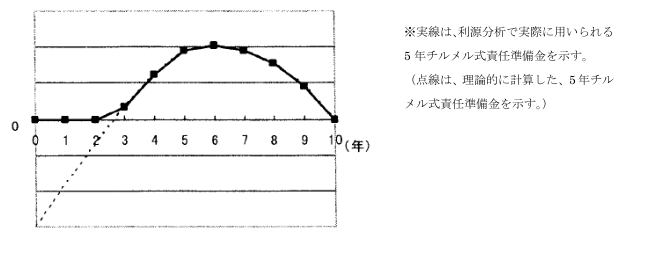
\includegraphics[scale=0.8]{images/ProbH15-2-2-2.png}

\answer{}

◯利源枠の説明

利源分析上、費差益の計算に用いる予定事業費枠。予定新契約費のうち一定割合を契
約初年度に費消し、それを一定期間で償却すると考えて計算した予定事業費枠である。
この予定新契約費の一定割合のことをチルメル歩合(α')といい、償却期間をチルメル
期間という。チルメル期間は、金融庁に報告する利源分析においては現在5年間とされ
ている。

また、チルメル歩合α'を営業保険料で賄いきれない場合、α'
の残りの部分を次年度以降順次費消するとして計算する
「限度超過修正」(または「Negative Reserve 修正」)
を行う。この結果、責任準備金が負値とならない。

利源枠のメリットとしては、
\begin{itemize}
\item[] 解約控除まで考慮に入れた財源対応では、より実態に近い
\item[] 保険料収入を限度とした枠計上である
\item[] 業界共通の尺度として採用されている
\end{itemize}

また、デメリットとしては、
\begin{itemize}
\item[] チルメル期間経過後、予定事業費が大きくなる点が不自然である
\item[] 2年目以降チルメル期間内の新契約費が通常マイナスとなる
\end{itemize}

○利源枠の図示

チルメル期間内における利源枠は、
$$
\text{蔵銀枠} + \alpha/\ax**{x:\angl{10}} - \alpha/\ax**{x:\angl{5}}  - \text{限度超過修正}
$$
ここで、蔵銀枠は、初年度は $\alpha+\delta\cdot P+\gamma+\beta\cdot P$である。

限度超過修正は、理論上の5年チルメル式責任準備金が負値となる期間が2年であることから、
調整は3年に亘ることがわかる.

チルメル期間終了後は、純保枠と一致する。

1年目
$$
\delta\cdot P + \gamma + \beta\cdot P + \alpha/\ax**{x:\angl{10}} - \alpha/\ax**{x:\angl{5}}
+\alpha+ vp_x\cdot\Vx[1]{x}[5z(*)]
$$

2年目
$$
\delta\cdot P + \gamma + \beta\cdot P + \alpha/\ax**{x:\angl{10}} - \alpha/\ax**{x:\angl{5}}
- \Vx[1]{x}[5z(*)]+ vp_{x+1}\cdot\Vx[2]{x}[5z(*)] 
$$

3年目
$$
\delta\cdot P + \gamma + \beta\cdot P + \alpha/\ax**{x:\angl{10}} - \alpha/\ax**{x:\angl{5}}
 - \Vx[2]{x}[5z(*)]
$$

4, 5年目
$$
\delta\cdot P + \gamma + \beta\cdot P + \alpha/\ax**{x:\angl{10}} - \alpha/\ax**{x:\angl{5}}
$$

6年目以降=純保枠と一致
$$
\delta\cdot P + \gamma + \beta\cdot P + \alpha/\ax**{x:\angl{10}} 
$$

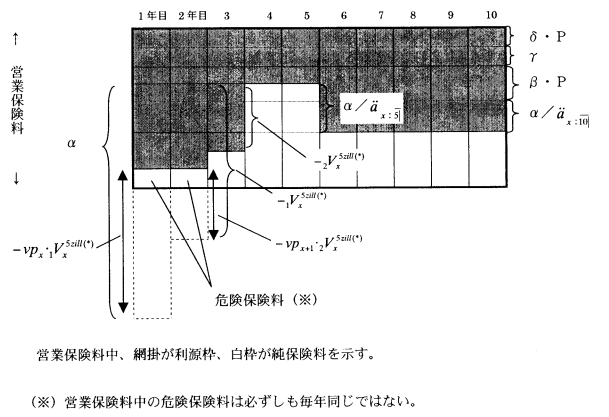
\includegraphics[scale=0.8]{images/ProbH15-2-2-2a.png}

\problem{H30 生保2問題 2(2)、H20 生保2問題 2(2)}
保険種類別に事業費効率を把握することの目的、結果の利用方法について簡潔に説明しなさい。
\answer{}
目的

\begin{itemize}
 \item[] 事業費の支出形態は、募集組織の違い等により個人保険や団体保険等で異なる点が多く、付加保
 険料の体系も異なったものが採用されている。また、個人保険内においても、販売チャネル・商
 品特性・払方の違い等により、事業費の支出形態や付加保険料体系の違いがある。
 \item[] 複数の保険種類を取り扱う場合、保険種類間の事業費効率の差異やそれぞれの改善度を把握する
 ことは、「付加保険料の合理性・妥当性の確保」、「契約者間の公平性の確保」、「保険会社の経営
 効率化」といった観点で重要である。
 \item[] ただし、予定事業費は保険種類別に把握することが可能である一方、事業費支出については、保
 険種類別の帰属が明確でない費用(総務部門人件費等)が存在するため、適切な配賦により事業
 費効率を把握することが求められる。
\end{itemize}
結果の利用方法

\begin{itemize}
 \item[] 付加保険料の合理性・妥当性の確保、契約者間の公平性の確保
\begin{itemize}
\item[] 営業保険料の十分性を確保するのみならず、付加保険料部分についてもセルフ・サポートする
 のが望ましい。ここで、付加保険料と事業費だけではなく、解約失効益(解約控除益)のうち
 新契約費の回収分を加えて十分性を確認することも考えられる。
\item[] 保険種類別の事業費効率のデータは、新商品の付加保険料や募集手数料(営業職員給与や代理
 店手数料)の設定に活用できる。さらに、販売後においては、事業費効率をモニタリングし、
 付加保険料の合理性、妥当性の事後検証に活用していく。このサイクルに則り、必要に応じて
 料率改定(十分性が満たされていない商品の付加保険料の引上げ等)を行うことも考えられる。
\item[] 保険種類別の事業費効率のデータは、契約者配当の設定にも活用できる。たとえば、保険種類
 間の事業費効率の違いについて、調整配当として還元することで、契約者間の公平性を図るこ
 とができる。
\end{itemize}
\item[] 保険会社の経営効率化
\begin{itemize}
\item[] 経営資源の適正配分に活用できる。例えば、以下が考えられる。
\begin{itemize}
 \item[] 事業費効率の悪化している保険種類について、事務効率改善策の検討
 \item[] 総合的に収益の高い商品について、販売量増大を目的とした更なる事業費投入(営業職員
 給与の引上げ等)
\end{itemize} 
\item[] 保険種類別の事業費効率の実績推移を今後の事業費予算に活かすことで、事業費支出の削減、
 業務運営の効率化を図る。また、これを保険料の引下げにつなげることも考えられる。
 \item[] これらの取組みを、PDCAサイクル(「販売計画・商品政策に基づく事業費予算の策定⇒事
 業費予算の執行⇒保険種類別事業費効率の把握⇒販売計画・商品政策の見直し(新商品開発・
 料率改定)」の流れ)として繰り返すことで、収益面・料率面での他社競争力確保に繋げてい
 くことができる。
\end{itemize}
\end{itemize}
(※)その他、
「監督当局による事業費モニタリング」
「将来シミュレーション(将来収支分析等)」
「商品別収益管理・商品別原価管理」等について触れていれば、必要に応じて加点を行った。

\section{5.5 収益管理と原価管理}
\problem{2021 生保2問題 1(6)、H27 生保2問題 3(2)①、H24 生保2問題 2(3)、H14 生保2問題 1(7)、H8 生保2問題 1(4)、H2 生保2問題 2(1)}\vspace{1zh}
生命保険会社における原価管理の目的と、商品別原価計算の概略および留意点について、簡潔に説
明しなさい。
\answer{}
<原価管理の目的>
\begin{itemize}
\item[] 商品別・部門別・顧客別等の収益性分析への反映
\item[] 価格政策への反映(商品の保険料および配当の決定)
\item[] 事務効率改善策への反映
\end{itemize}

<商品別原価計算の概略および留意点>
商品別原価計算とは、費差損益対象経費を費目別に分類し、最終的には各商品に配賦するととも
に、それらの経費を適切な単位比例(例:保険金額あたり、営業成績あたり、保険料あたり、一件
あたり等。これらの単位を「コスト分母」という)のコストとして把握することをいう。

商品別原価計算をおこなうことによって、商品別の事業費支出状況を把握することが可能となり、
商品政策、価格政策、販売政策等を策定する際に実施する将来収支計算(シミュレーション)に活
用することができる。

商品別原価計算の手法(手順)の概要は次のとおりである。

\begin{enumerate}[i]
\item[] 費目別分類\\
 費差損益対象経費を適切な費目に区分する。\\
 対象経費については、死差損益に係る費用(契約加入時の診査経費、契約確認経費および保険金
 給付金支払い請求時の契約確認経費)、利差損益に係る費用(投資関係費用)、および狭義の事業
 費に属さない費用(契約関係税金、減価償却費および退職給付引当金繰入額等)を対象とするか
 否かを明確にする。\\
 区分にあたっては、以下の観点に留意する。
\begin{itemize}
\item[] 初年度費用と次年度以降費用の区分
\item[] 固定費・変動費の区分
\item[] 払方別経費
\item[] 診査方法別経費・集金経路別経費、販売チャネル別経費、営業職員資格別経費 等
\end{itemize} 
\item[] 商品別分類\\
 費目別に分類した経費を個人保険(各商品別)、企業保険(各商品別)等に分類する。費用が商品
 別に直接区分されていることは少なく、ほとんどの場合、何らかの配賦により商品別費用を求め
 ることになる。\\
 配賦基準(保険金額、営業成績、新契約件数、保有件数、処理件数、給与、作業延べ時間、職員
 数、コンピュータ処理時間等)を定める際、通常は消費主義(実態として、何に比例して支出さ
 れているかに基づくもの)によるべきであるが、負担能力主義(本来、何に比例して負担すべき
 ものかに基づくもの)によらざるをえない場合もある。
\item[] コスト分母別把握\\
 経費が何に比例して支出されているかに基づき、費目毎にコスト分母(保険金額、営業成績、
 新契約件数、保有件数、保険料、責任準備金等)を決定する。複数のコスト分母に比例させる
 場合もあり得る。
\item[] コスト係数計算\\
 コスト分母別に把握した経費を対応するコスト分母にて除してコスト係数を計算する。コスト係
 数が算出されて初めて商品別の将来収支シミュレーションが可能となる。
\end{enumerate}

\section{5.6 事業費と生命保険会社の経営}
\problem{2020 生保2問題 1(4)}
金融庁による事業費モニタリングについて、以下の①~⑤の空欄に当てはまる適切な語句を記入
しなさい。

\noindent ○「5-7\wakumaru{①}の充足状況」

保険種類・\wakumaru{②}
の区分ごとの新契約に係る事業費の効率等を見る資料で、定期的に
金融庁宛報告を要する。報告対象は、原則として、当該期における新契約の全て。

\wakumaru{①}に関して、保険種類および\wakumaru{②}の区分ごとに、
「\wakumaru{③}」、「事業費」、「\wakumaru{④}」を算出し、
「効率(事業費÷\wakumaru{③})」および「回収予定平均年数(事業
費÷\wakumaru{④})」を報告する。

\noindent ○「5-9 \wakumaru{⑤}の充足状況」

保険種類・\wakumaru{②}
の区分ごとの契約維持・管理のために支出する事業費の回収状況を
見る資料で、定期的に金融庁宛報告を要する。報告対象は、当該期における全保有契約。
\answer{}
\begin{itemize}
\item[ ①: ] イニシャルコスト
\item[ ②: ] 販売経路
\item[ ③: ] 予定事業費現価
\item[ ④: ] 年換算予定事業費
\item[ ⑤: ] ランニングコスト
\end{itemize}

\problem{H19 生保2問題 3(2)①、H5 生保2問題 2(2)}
生命保険会社における特徴的な経費である新契約費の持つ会計的意味(収入と支出の特徴)につい
て、簡潔に説明せよ。
\answer{}
一般の商品であれば、その商品の販売による代金の回収(収益の計上)は短期間の
内に完了するところであり、販売に要した費用と収益を同時期に計上することが、通常
平易である。このように、一般には費用は収益と対応させて認識することとなっている
が、生命保険会社における収益は、月々あるいは毎年収入される保険料収入により実現
するところであり、これを費用とどのように対応させるかという点に大きな特徴がある。

新契約に要する費用は営業職員にかかる経費を中心に契約初期にある程度集中して
発生するのが普通であり、一方、これに充てる付加保険料は、契約が継続する間の収入
保険料中に含まれている。このために、新契約経費対付加保険料、すなわち費用対収益
の対応を合理的にコントロールするために、予定事業費枠の考え方が種々考案されてい
る。それぞれ会計的な意味合いや妥当な効率評価での意味合いに長所・短所があり、保
険会社はそれを踏まえて経営上の基準として使用している。

新契約関係のコスト構造への対応は、生命保険会社における事業費管理の一つのポイ
ントであり、生命保険経営において常に検討を続けなければならない。

初年度経費が償却されないまま契約が消滅するというケースに対しては、例えば、継
続率改善を図るという対応や、人件費支出の構造自体を新契約の一時点に集中させるの
ではなく、保険契約の継続状況に応じて支出するという対応がある。

\problem{H22 生保2問題 1(1)}
金融庁による事業費モニタリングの概要に関し、以下の①~⑤の空欄に当てはまる適切な語句を記
入しなさい。

各生命保険会社は、イニシャルコストの負担方法(分割負担年限等)、イニシャルコストを回収する
ための\wakumaru{①}
の収納方法(契約時に一時に収入か平準的に収入か等)などの差異を勘案して報告する
単位としての\wakumaru{②}
および保険種類の区分を設定し、イニシャルコスト・ランニングコストに区分し
て各種の事業費支出状況・\wakumaru{①}
収入状況を金融庁に定期的に報告しなければならない。特にイニシ
ャルコストの回収状況およびランニングコストの\wakumaru{③}
状況のモニタリングに主眼が置かれている。

ここで、イニシャルコスト・ランニングコストとは、
\begin{itemize}
\item[]  イニシャルコスト:\wakumaru{④}のために支出する事業費
\item[]  ランニングコスト:\wakumaru{⑤}のために支出する事業費で、イニシャルコストとして把握する項目以外の事業費
\end{itemize}
を意味し、各社が実態に即して適宜設定することとなっている。
\answer{}
\begin{itemize}
\item[①: ] 予定事業費
\item[②: ] 販売経路
\item[③: ] 充足
\item[④: ] 新契約獲得
\item[⑤: ] 契約維持・管理
\end{itemize}

\problem{H28 生保2問題 1(4)}
金融庁による事業費モニタリングについて、以下の①~⑤の空欄に当てはまる適切な語句を記入しな
さい。

○生命保険会社は、平成 18 年 4 月以降、次の 5 つの資料を金融庁宛定期報告することとなっている。
\begin{itemize}
\item[] 5-5 「予定事業費等の設定状況」
\item[] 5-6 「総合的な充足状況」
\item[] 5-7 「\wakumaru{①}の充足状況」
\item[] 5-8 「\wakumaru{①}の回収状況」
\item[] 5-9 「\wakumaru{②}の充足状況」
\end{itemize}

○「\wakumaru{①}の充足状況」について

保険種類および\wakumaru{③}
の区分ごとの新契約に係る事業費の効率等を見る資料で、定期的に金融庁宛
報告を要する。報告対象は、原則として、当該期における新契約の全て。
\wakumaru{①}に関して、保険種類および\wakumaru{③}の区分ごとに、
「\wakumaru{④}」、「事業費」、「\wakumaru{⑤}」を算出し、
「効率(事業費÷\wakumaru{④})」
および「回収予定平均年数(事業費÷\wakumaru{⑤})」を報告する。

\answer{}
\begin{itemize}
\item[ ①: ]  イニシャルコスト
\item[ ②: ]  ランニングコスト
\item[ ③: ]  販売経路
\item[ ④: ]  予定事業費現価
\item[ ⑤: ]  年換算予定事業費
\end{itemize}

\problem{H25 生保2問題 2(3)}
金融庁による事業費モニタリングについて、導入された背景および概要を簡潔に説明しなさい。
\answer{}
<導入の背景>
\begin{itemize}
 \item[] 金融庁は、保険会社の経営効率化への取組み等の経営努力を保険料に適時適切に反映させる
 観点から、保険料のうち保険数理に直接よらない部分を中心に商品審査を簡素化するととも
 に、事業費に関する充実したモニタリングを行うことにより、監督の実効性の向上を図り、
 保険料の合理性・妥当性・公平性を確保した上で、保険商品の価格の弾力化を推進するため
 に、2006 年 2 月に「保険業法施行規則」および「保険会社向けの総合的な監督指針」を改
 正(実施日は 2006 年 4 月 1 日)した。
 \item[] これにより、保険料及び責任準備金の算出方法書の記載事項から「予定事業費に関する事項」
 が削除され、予定事業費の算出方法は社内規程等に定めることとなる一方、金融庁が事業費
 の実績と保険料の関係を把握するために、各生命保険会社は事後モニタリングとして、商品
 別等に細分化した定期報告を金融庁に提出することとなった。
\end{itemize}
<概要>
\begin{itemize}
 \item[] 各生命保険会社は、イニシャルコストの負担方法、イニシャルコストを回収するための予定
 事業費の収納方法などの差異を勘案して報告する単位としての販売経路および保険種類の
 区分を設定し、イニシャルコスト・ランニングコストに区分して各種の事業費支出状況・予
 定事業費収入状況を金融庁に定期的に報告しなければならない。特に、イニシャルコストの
 回収状況およびランニングコストの充足状況のモニタリングに主眼が置かれている。
 \item[] イニシャルコストは「新契約獲得のために支出する事業費」、ランニングコストは「契約維持・
 管理のために支出する事業費で、イニシャルコストとして把握する項目以外の事業費」を意
 味し、各社が実態に則して適宜設定することとなっている。
 \item[] 金融庁に提出する資料は次の5つである。
 \begin{itemize}
 \item[] 「5-5 予定事業費等の設定状況」:保険種類・特約種類ごとに予定事業費・解約控除の
 設定方法を記載。新商品発売時、または予定事業費・解約控除の設定を変更した都度、翌
 月に報告する。
 \item[] 「5-6 総合的な充足状況」:イニシャルコスト・ランニングコストの充足状況を総括的
 に見るための資料。年単位で報告する。
 \item[] 「5-7 イニシャルコストの充足状況」:保険種類・販売経路区分ごとの新契約に係る事
 業費の効率等を見る資料。四半期毎に報告する。\\
 具体的には、「①予定事業費現価」、「②事業費」、「③年換算予定事業費」を算出し、「効率
 (②÷①)」および「回収予定平均年数(②÷③)」を報告する。
 \item[] 「5-8 イニシャルコストの回収状況」:保険種類・販売経路区分ごとの新契約に係る事
 業費の、解約控除を考慮した回収状況を見る資料。年単位で報告する。\\
 具体的には、最大過去5年間分について、契約事業年度単位で、「5-7 イニシャルコス
 トの充足状況」を年度単位にまとめたものの他、「⑦予定事業費」、「⑧事業費」、「⑨解約控
 除・消滅契約未回収残高」、「⑩未回収残高」および「回収見込年数」を報告する。
 \item[] 「5-9 ランニングコストの充足状況」:保険種類・販売経路区分ごとの契約維持・管理
 のために支出する事業費の回収状況を見る資料。年単位で報告する。\\
 具体的には、最大過去5年間分について、契約事業年度単位で、「⑪予定事業費」、「⑫事
 業費」および「収支(⑪-⑫)」を報告する。
 \end{itemize}
\end{itemize}
%Anki kokomade
\end{document}